\documentclass{article}
\usepackage[utf8]{inputenc}
\usepackage[english]{babel}
\usepackage[document]{ragged2e}
\usepackage{graphicx}

\title{loss}
\author{Grand Maxence}
\date{\today}

\begin{document}
\maketitle
\begin{figure}[!h]
  \centering
  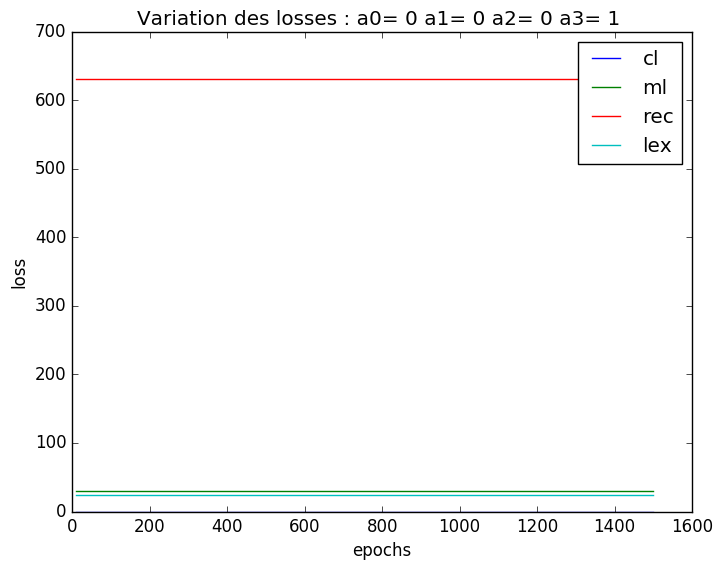
\includegraphics[scale=0.8]{img/loss/test1.png}
  \caption{Test 1}
\end{figure}
\begin{figure}[!h]
  \centering
  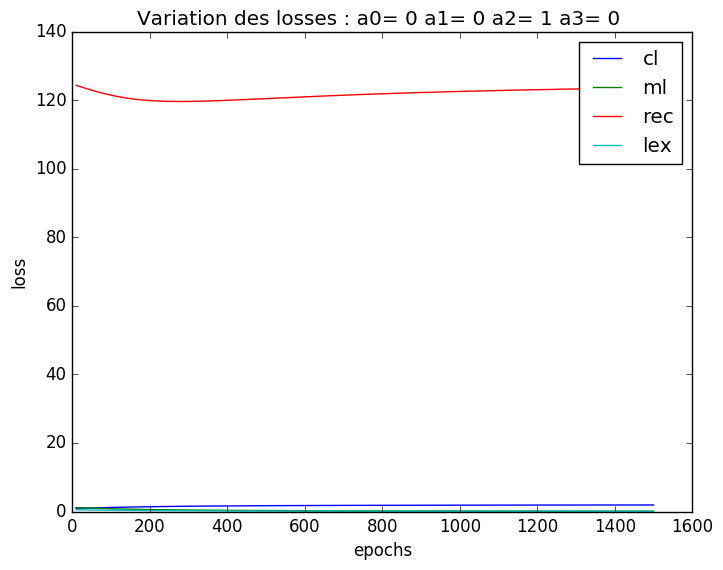
\includegraphics[scale=0.8]{img/loss/test2.png}
  \caption{Test 2}
\end{figure}
\begin{figure}[!h]
  \centering
  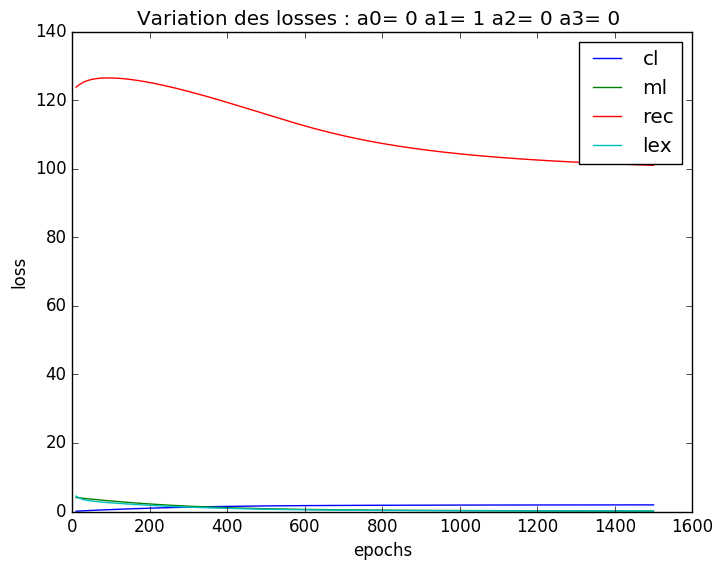
\includegraphics[scale=0.8]{img/loss/test3.png}
  \caption{Test 3}
\end{figure}
\begin{figure}[!h]
  \centering
  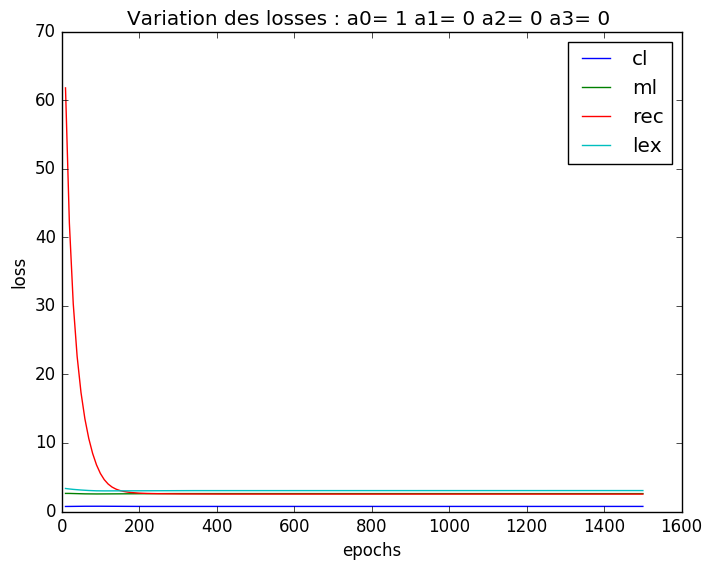
\includegraphics[scale=0.8]{img/loss/test4.png}
  \caption{Test 4}
\end{figure}
\begin{figure}[!h]
  \centering
  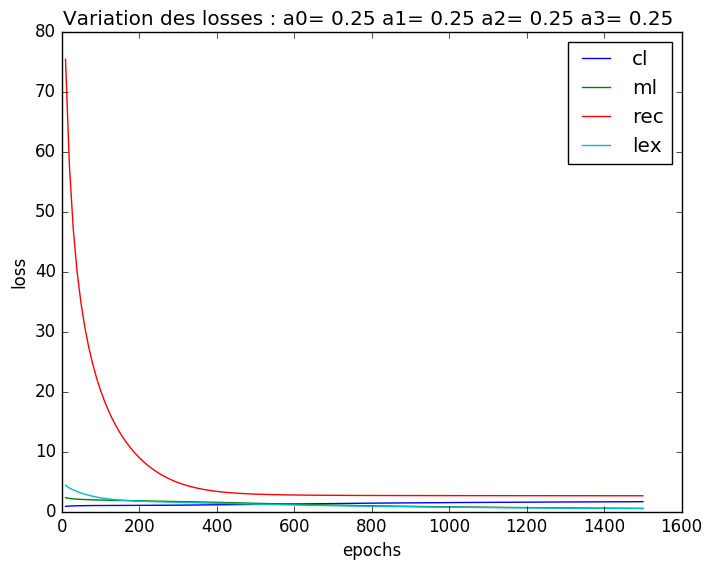
\includegraphics[scale=0.8]{img/loss/test5.png}
  \caption{Test 5}
\end{figure}
\begin{figure}[!h]
  \centering
  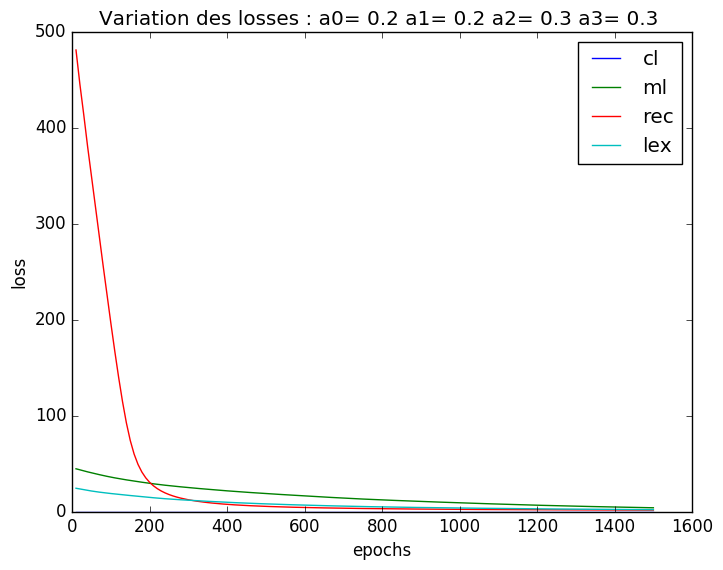
\includegraphics[scale=0.8]{img/loss/test6.png}
  \caption{Test 6}
\end{figure}
\begin{figure}[!h]
  \centering
  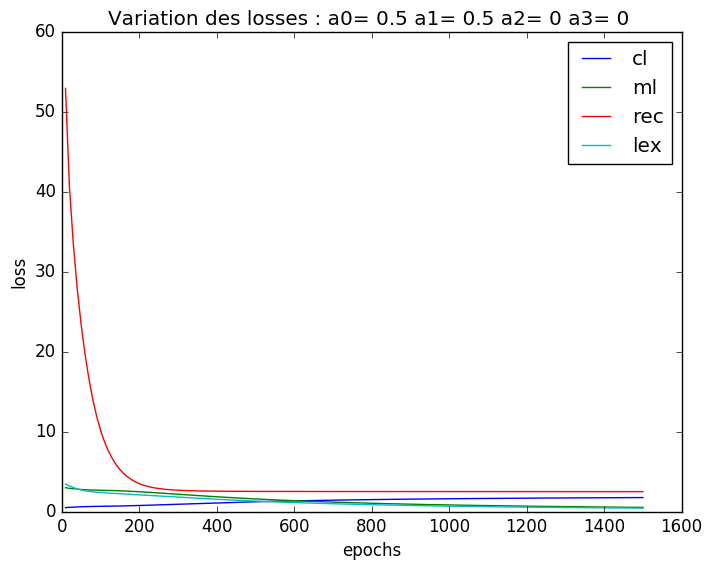
\includegraphics[scale=0.8]{img/loss/test7.png}
  \caption{Test 7}
\end{figure}
\begin{figure}[!h]
  \centering
  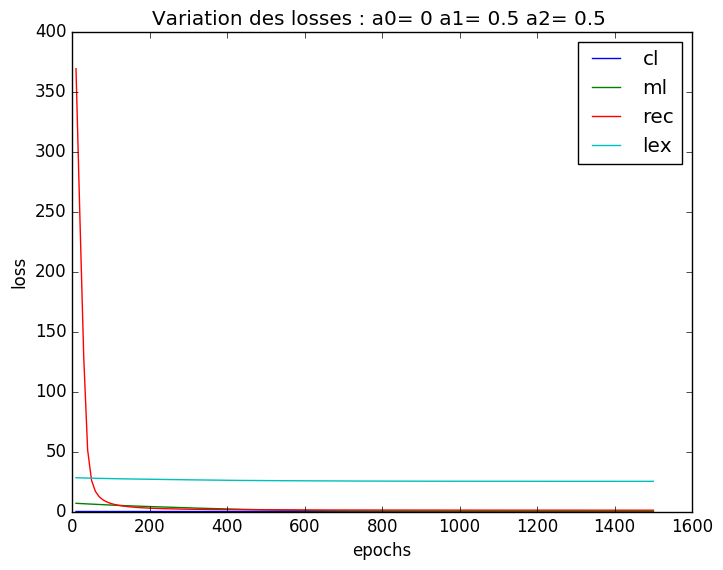
\includegraphics[scale=0.8]{img/loss/test8.png}
  \caption{Test 8}
\end{figure}
\begin{figure}[!h]
  \centering
  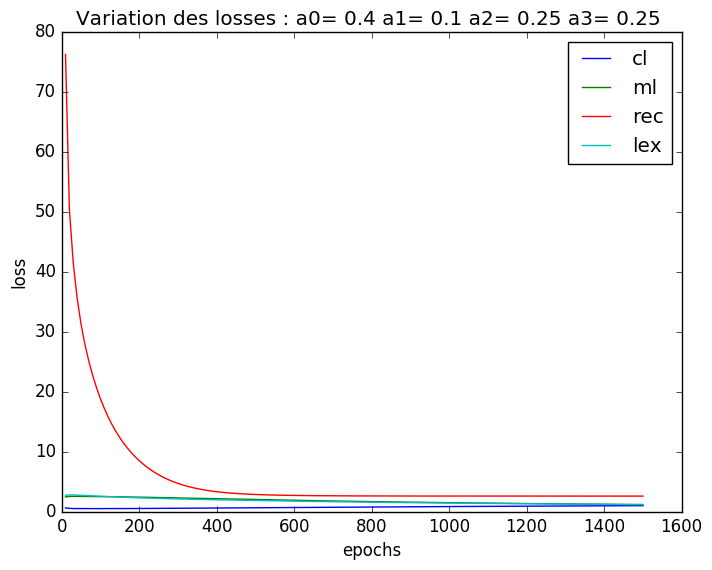
\includegraphics[scale=0.8]{img/loss/test9.png}
  \caption{Test 9}
\end{figure}
\begin{figure}[!h]
  \centering
  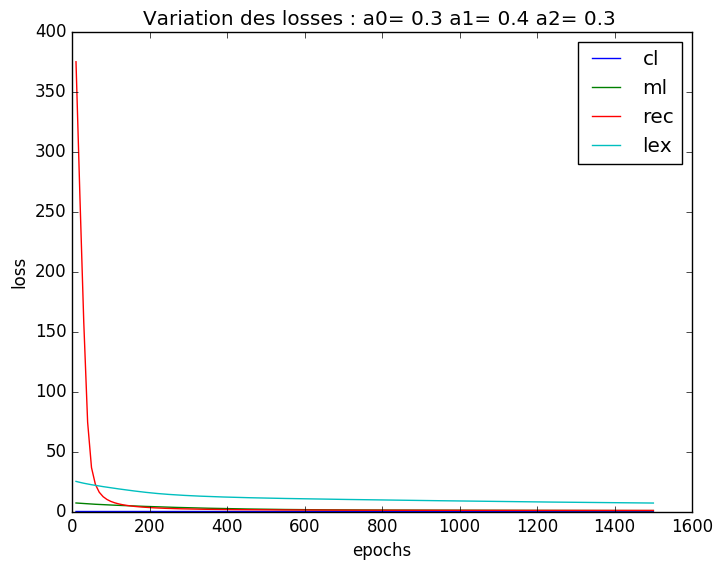
\includegraphics[scale=0.8]{img/loss/test10.png}
  \caption{Test 10}
\end{figure}
\end{document}